\section{Applications}\label{sec:applications}

In  this section, we show some applications of our results in the context of a DoS analysis of DNS. We present the examples informally, showing how instances of security properties can be characterized as $\mathsf{FO}(<)$-properties, and translating the security analysis to an instance of the $\verif$ problem. We further demonstrate how we can compute the abstractions of the inputs of the $\verif$ instance using syntactic domain congruence.


\begin{figure}
    \subfloat[\new{An illustration of the NXNSAttack.}]{
    \label{subfig:nxns-illustration}
    \centering
   \resizebox{0.6\textwidth}{!}{\includegraphics[width=\textwidth]{img/dns-amp.pdf}}
    }
\hfill
    \subfloat[\new{The zone configuration. We omit the redundant components (for this attack).}]{
    \label{subfig:nxns-zone}
    \centering
   \resizebox{0.35\textwidth}{!}{
    \begin{tikzpicture}[every label/.style={font=\small}]
				\node (before) [fill=blue!5,draw,rounded corners=2pt, label=north:\emph{Concrete Zone}] at (0,0) {
					\begin{tabular}{l} 
						--- \textbf{zone} \emph{net.attacker} ---\\
						$\tup{net.attack.nxns,\scrsf{ns},net.victim.nx1}$\\
						$\tup{net.attack.nxns,\scrsf{ns},net.victim.nx2}$\\
						$\tup{net.attack.nxns,\scrsf{ns},net.victim.nx3}$\\
					\end{tabular} };
				\node (after) [fill=olive!10,draw,rounded corners=2pt, label=south:\emph{Abstract Zone}] at (0,-3) {					
				\begin{tabular}{l} 
						--- \textbf{zone} $\synhom{\scrsf{nxns}}(net.victim)$ ---\\
						$\tup{\synhom{\scrsf{nxns}}(net.attack.nxns),\scrsf{ns},\synhom{\scrsf{nxns}}(net.victim.nx1)}$\\
						$\tup{\synhom{\scrsf{nxns}}(net.attack.nxns),\scrsf{ns},\synhom{\scrsf{nxns}}(net.victim.nx2)}$\\
						$\tup{\synhom{\scrsf{nxns}}(net.attack.nxns),\scrsf{ns},\synhom{\scrsf{nxns}}(net.victim.nx3)}$\\
				\end{tabular} };
				\draw [double distance=2pt, -{Implies}, shorten <= 2pt, shorten >= 2pt] (before) -- (after) node [midway, right] {$\synhom{\scrsf{nxns}}$};
	\end{tikzpicture}}
    }
\hfill
    \subfloat[
    	A local run in the process $\rec{r}$ in $\scrsf{dns}\subsub{\scrsf{nxns}}$ that corresponds to Figure \ref{subfig:nxns-illustration}. In the initial configuration, the server list $sl_0 = (net.attacker)\odot (net.victim)$ contains the domain names of the other two nameservers, and the initial cache $cache_0 = \{\tup{net.attacker,\scrsf{a},5.6.7.8},\tup{net.victim,\scrsf{a},1.2.3.4}\}$ contains the IP addresses of both these nameservers. For notational convenience, we use $('')$ in a configuration to represent the corresponding component unchanged from the previous configuration; we use $(*)$ to represent a timer valuation after an arbitrary elapse of time; the transitions with labels in \{\ding{183},...,\ding{190}\} informally correspond to the messages in \Cref{subfig:nxns-illustration}, omitting the associated stack operation annotations.  We also drop the messages \ding{182} and \ding{191} as we do not model the client in our model. Instead, the message \ding{182} is represented by the internal transition $\tup{\epsilon, in, \tup{net.example,\scrsf{a}}}$. The messages \ding{186},\ding{188},\ding{190} are replaced by $\tup{\scrsf{nxdomain},\emptyset}$ in the model.
    	]{
    \label{subfig:nxns-run}
    \begin{minipage}[b]{\linewidth}
    \centering
       \includegraphics[width=\textwidth, page=2]{img/formal-run-nxns-crop.pdf}
    \end{minipage}
    }
    \captionsetup{skip=5pt}
\caption{\label{fig:nxns}\new{NXNSAttack.}}
\end{figure}


\subsection{Amplification Attacks}\label{subsec:amplification}

An \emph{amplification attack} is a type of DoS attack where an attacker exploits DNS to overwhelm a target, such as  resolvers and nameservers, with a large volume of traffic, effectively disrupting its ability to function.
For example,
in the recently discovered NXNSAttack (NoneXistent Name Server Attack)~\cite{NXNSAttack}, a small DNS query triggers the DNS resolver to issue a much larger response, potentially achieving a packet amplification factor (PAF) of over a thousand times  the original query size.

Let us first have a closer look at amplification attacks. Informally, given a ZFC $\tup{\cal Z, \Theta}$, a target process $p$, and an amplification factor $\mathit{paf} \in \nat$, the corresponding instance of DNS exhibits an amplification attack if there exists some query that, during the query resolution process, causes the target process $p$ (either a nameserver or a resolver) in the network to receive more than $\mathit{paf}$ messages. Typically, the target process refers to a nameserver in the network which, for a sufficiently large $\mathit{paf}$, is then unable to respond to legitimate query requests. In order to discover amplification attacks, one must exhaustively analyze all possible DNS behaviours, \emph{for every query}, and check if there exists a behaviour where a target nameserver receives more than $\mathit{paf}$ messages.

Borrowing notation from earlier sections, we can formally characterize the set of traces that exhibit an amplification attack as the formula,\footnote{We use many-sorted quantification in the formula, in order to quantify over the space of all messages in $\mathsf{M}\subsub{\cal Z}$, which is an infinite set. The alternative would be an infinite disjunction over all possibilities of $\mathit{msg}$.}

\begin{equation*}\label{eqn:amp-prop}
\resizebox{\textwidth}{!}{$\phi_{amp}(\mathit{paf},p) = \exists x_1,\ldots,x_{\mathit{paf}}\in \nat.\, \left(\bigwedge\limits_{i\neq j \in \{1,\ldots ,\mathit{paf} \}} x_i \neq x_j\right)  \wedge \left( \bigwedge\limits_{i\in \{1,\ldots , \mathit{paf} \}}\bigvee\limits_{j \in P\subsub{\cal Z}} \left(\exists \mathit{msg}\in \mathsf M\subsub{\cal Z}.(\ch_{(j,p)}?\mathit{msg})(x_i)\right) \right)$}
\end{equation*}


The above formula captures the property that there exist $\mathit{paf}$ distinct positions in a trace, such that every one of these positions corresponds to a receive action for the target process $p$. Indeed, any run in $\scrsf{dns}\subsub{\cal Z}$ whose trace satisfies the above property exhibits a receive action for the target component $\cal P^p$ at least $\mathit{paf}$ times. Since every run in $\scrsf{dns}_{\cal Z}$ begins with a query request, a run that satisfies $\phi_{amp}(\mathit{paf},p)$ corresponds to an amplification attack.

\new{
\begin{example}
 Figure~\ref{subfig:nxns-illustration} illustrates how the NXNSAttack is mounted using a simple example.
 This example involves two attacker components, namely a client and an authoritative nameserver \name{attacker.net}, and two innocent components, namely the recursive resolver and an authoritative nameserver \name{victim.net}. 
The client issues a request 
for the subdomain \name{nxns.attack.net} that
is authorized by the attacker's authoritative nameserver (\ding{182}). 
The resolver then attempts to  resolve the subdomain  (\ding{183}).
In response, the attacker's nameserver 
\name{attacker.net}
sends an \rtype{ns} 
referral response with multiple nameserver names (three in this case) but without their IP addresses 
(\ding{184}).
This forces the resolver to issue additional  subqueries to resolve each of these names (\ding{185}--\ding{190}), thus amplifying the DNS traffic.

The ZFC can be represented by $\tup{\scrsf{nxns},\{5.6.7.8,1.2.3.4\}}$, where the domain of $\scrsf{nxns}$ is the set $\{5.6.7.8,1.2.3.4\}$, such that $5.6.7.8$ is the IP of the attacker's nameserver and $1.2.3.4$ that of the victim. The function $\scrsf{nxns}$ essentially\footnote{For simplicity, we only consider the records that are relevant for the attack.} maps $1.2.3.4$ to the empty set and $5.6.7.8$ to the concrete zone illustrated in \Cref{subfig:nxns-zone}. The malicious zone contains three $\scrsf{ns}$ records that point to the nameservers with domain names $net.victim.nx\{i\}$, for $i \in \{1, 2, 3\}$. But, observe that none of them have an accompanying record of type $\scrsf{a}$ that points those names to an IP address. The IP addresses $1.2.3.4$ and $5.6.7.8$ are recorded as the root nameserver IP addresses. 

We now describe the run of the resolver in $\scrsf{dns_{nxns}}$. The resolver starts from the initial configuration, and takes the internal transition with the label $\tup{\epsilon, in, \tup{net.attacker.nxns,\scrsf{a}}}$ to model that it received the query $\tup{net.attacker.nxns,\scrsf{a}}$ from the client. When it \emph{receives} the query, it moves to the $query$ state ready to start resolution. The current stack configuration is $\tup{net.attack.nxns,\scrsf{a}}$, which denotes that the initial query is currently under the resolution. It then sends the query out to the leftmost nameserver in the server list that contains the domain name of the query in its zone, namely $attacker.net$, and then waits for an answer by moving to the state $wait$. Once it receives the response with a set of  $\scrsf{ns}$ records from $\ns{5.6.7.8}$, it adds them to its cache, along with the corresponding domain name of the nameserver in the value of each record (in the answer) to its server list. It moves back to the $query$ state to decide the next step for the resolution. Since every $\scrsf{ns}$ record in the answer was glueless, the resolver proceeds with the resolution of $\tup{net.victim.nx1,\scrsf{a}}$ in order to find the glue. Consequently, it pushes the query on its stack while staying in the $query$ state. Since the query name is in the zone $victim.net$, it sends the query to $\ns{1.2.3.4}$. However, since the zone file for $victim.net$ is empty, the resolver gets $\tup{\scrsf{nxdomain},\emptyset}$ (\ding{186}) as the answer, thus deleting $net.victim.nx1$ from its server list and moving back to the $query$ state. This repeats two more times for the other two entries in the server list. It is then straightforward to see that this behaviour leads to $\ns{1.2.3.4}$ receiving three queries. In fact, this behavioural pattern can be easily extended such that $\ns{1.2.3.4}$ receives $n$ queries for any $n \in \nat$, by adding more records of the form $\tup{net.attack.nxns,\scrsf{ns},net.victim.nx\{i\}}$ to the zone $attack.net$. \Cref{subfig:nxns-run} illustrates the formal run in the process $\rec{r}$.






The PPT languages required to compute the abstraction are $L_0 = net\cdot attack\cdot nxns \cdot \dnsAlph^+$, and $L_i = net\cdot victim\cdot nx\{i\}\cdot \dnsAlph^+$, where $\dnsAlph = \{net, attack, nxns, 1, 2, 3, other\}$ and $i \in \{1, 2, 3\}$. We  compute the monoid $\scrsf{syn}\subsub{\scrsf{nxns}} = \prod_{0 \leq j \leq 3}\tup{\synmon{L_j}}$, denoting the sytactic domain congruence classes and the corresponding homomorphism $\synhom{\scrsf{nxns}}$. Fixing the packet amplification factor to be $3$ and the target process to be $1.2.3.4$, the formula $\phi_{amp}(3, 1.2.3.4)$ can then be rewritten as

\begin{equation*}\label{eqn:amp-prop}
\resizebox{\textwidth}{!}{$\phi_{amp}'(3,1.2.3.4)  = \exists x_1,\ldots,x_{3}\in\nat.\, \left(\bigwedge\limits_{i\neq j \in \{1,\ldots ,3 \}} x_i \neq x_j\right)
	 \wedge \left( \bigwedge\limits_{i\in \{1,\ldots , 3 \}}\bigvee\limits_{j \in \{r,5.6.7.8\}}\bigvee\limits_{\stackrel{m \in \scrsf{syn}\subsub{\scrsf{nxns}},}{t \in \scrsf{type}}} (\ch_{(j,1.2.3.4)}?\tup{m,t})(x_i)\right)$},
\end{equation*}


\noindent which no longer contains any quantifications other than the positions in the trace. The zone can be translated as shown in \Cref{subfig:nxns-zone}.
\end{example}
}

\paragraph{Unbounded Analysis}
Note that, if there are multiple nameservers, unlike the trivial example given above, there is no limit to the length of runs which can ensure the presence or absence of an amplification attack. Indeed, a resolver may communicate with the same benign nameserver owning multiple zones before establishing communication with the target nameserver. Hence, a complete search for amplification attacks necessitates the unbounded reachability analysis of $\scrsf{dns}$.


\begin{figure}
\label{fig:blackholing}
    \subfloat[\new{An Illustration of rewrite blackholing.}]{
    \label{subfig:blackholing-illustration}
    \centering
   \resizebox{0.55\textwidth}{!}{\includegraphics[width=\textwidth]{img/dns-blackholing.pdf}}
    }
\hfill
    \subfloat[\new{The concrete zone configuration.}]{
    \label{subfig:blackholing-zone}
    \centering
   \resizebox{0.4\textwidth}{!}{
    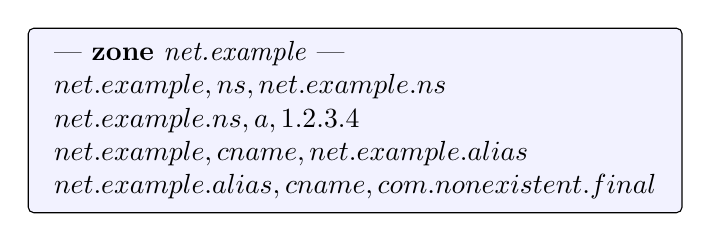
\begin{tikzpicture}[every label/.style={font=\small}]
            \node (before) [fill=blue!5,draw,rounded corners=2pt] at (0,0) {
                \begin{tabular}{l} 
                    --- \textbf{zone} \emph{net.example} ---\\
                    $\tup{net.example,\scrsf{ns},net.example.ns}$\\
                    $\tup{net.example.ns,\scrsf{a},1.2.3.4}$\\
                    $\tup{net.example,\scrsf{cname},net.example.alias}$\\
                    $\tup{net.example.alias,\scrsf{cname},com.nonexistent.final}$\\
                \end{tabular} };
    \end{tikzpicture}}
    }
\hfill
    \subfloat[\new{A local run of the process $\rec{r}$ that corresponds to Figure \ref{subfig:blackholing-illustration}. In the initial configuration, the server list $sl_0 = (net.example.ns)\odot (com)$ contains the domain names of the other two nameservers, and the initial cache $cache_0 = \{\tup{net.example.ns,\scrsf{a},1.2.3.4},\tup{com,\scrsf{a},0.0.0.0}\}$ contains the IP addresses of both these nameservers. We follow the notational conventions from the previous example (see \Cref{subfig:nxns-run}).
    }]{
    \label{subfig:blackholing-run}
    \begin{minipage}[b]{\linewidth}
    \centering
       \includegraphics[width=\textwidth, page=2]{img/formal-run-blackholing-crop.pdf}
    \end{minipage}
    }
    \captionsetup{skip=5pt}
\caption{\new{Rewrite blackholing.}}
\end{figure}

\subsection{Rewrite Blackholing}\label{subsec:rewrite-black}


\new{
\emph{Rewrite blackholing} occurs when a query is eventually redirected to a non-existent domain name. 
This can happen when the resolver, for example, follows some \rtype{cname} records, but ultimately finds that the final ``canonical'' name does not exist.
While rewrite blackholing can be useful for blocking malicious traffic or preventing attacks, it can also be exploited to blackhole legitimate services or domains, thus
 causing a DoS for valid queries.
}

\new{We now show that this attack vector can also be specified in our framework. Informally, given a ZFC $\tup{\cal Z, \Theta}$, the corresponding instance of DNS exhibits rewrite blackholing if there exists some query that, during its resolution process, causes the resolver to eventually receive an answer with the label $\scrsf{nxdomain}$ along with a non-empty set of records. 

We can again formally characterize the set of traces  exhibiting rewrite blackholing as the formula 
\begin{equation*}\label{eqn:rb-prop}
	\phi_{rb} = \exists x\in \nat.\exists recs \in \cal P(\scrsf{record}\subsub{\cal L}). \, \left(recs \neq \emptyset \wedge \bigvee_{j \in P\subsub{\cal Z}} \left((\ch_{(j,p)}?\tup{\scrsf{nxdomain},recs})(x_i)\right) \right).
\end{equation*}}

\new{
\begin{example}
As illustrated in Figure \ref{subfig:blackholing-illustration}, 
a DNS query for \name{example.net} returns a \rtype{cname} pointing to \name{alias.example.net} (\ding{184}). The resolver then queries \name{alias.example.net}, which returns another \rtype{cname} pointing to \name{final.nonexistent.com} (\ding{186}). Since \name{final.nonexistent.com} does not exist, the resolver eventually receives an \rtype{nxdomain} response, indicating that the domain cannot be resolved (\ding{188}). 
In this rewrite blackholing scenario,
two authoritative nameservers are involved: 
one  for handling the resolution of   
\name{example.net} and \name{alias.example.net}
(as both are within the same domain zone \name{example.net}), and the other for \name{nonexistent.com}. The concrete zone file for the \name{example.net} domain is shown in Figure~\ref{subfig:blackholing-zone} and the corresponding formal run in $\rec{r}$ is illustrated in \Cref{subfig:blackholing-run}.
\end{example}
}


